\documentclass[letterpaper,9pt]{article}

\usepackage{fullpage,amsmath,amsfonts,latexsym,xcolor,clrscode3e}
\usepackage{graphicx}
\usepackage{amsthm}
\usepackage{hyperref}
\usepackage{fullpage}
\usepackage[ruled,vlined,linesnumbered]{algorithm2e}

\usepackage{subcaption}
\usepackage{caption}
\usepackage{geometry}
\geometry{margin=.5in}

\graphicspath{ {./images/} }

\newcommand{\re}{{\mathbb{R}}}
\newcommand\numberthis{\addtocounter{equation}{1}\tag{\theequation}}
\newcommand{\floor}[1]{\lfloor {#1} \rfloor}
\newcommand{\ceil}[1]{\lceil {#1} \rceil}
\newcommand{\paren}[1]{\left( {#1} \right)}
\newenvironment{solution}{\color{black} }{}

\newcommand{\nats}{\mathbb{N}}

\newcommand{\comment}[1]{$\rhd$\ {\small\sf #1}}

\newtheorem{theorem}{Theorem}
\newtheorem{claim}[theorem]{Claim}
\newtheorem{lemma}[theorem]{Lemma}
\newtheorem{problem}{Problem}


%\begin{document}
%{\noindent\large
%{\em Introduction to Analysis of Algorithms} \hfill \today\\
%Boston University \hfill CS 330\\
%Professor  Adam Smith, Dora Erdos \hfill Fall 2020\\}
%\vspace{1pt}
%\hrulefill\vspace{3mm}
%\begin{center}
%{\LARGE\bf Programming Assignment 1}\\
%{\bf Due October 24, 2020 at 11:59 PM}
%\end{center}
%
%\begin{center}
%   Student: Justin DiEmmanuele
%\end{center}


\begin{document}
\section{Grid Graph Analysis}
\begin{enumerate}
    \item \textbf{$G^{1}_{gr}$ and $G^{4}_{gr}$ Infected Nodes and Probability Distribution}

    For the two grid graphs, the infected node count is shown below for each 
    probability level.

    %\begin{table}[htpb]
        %\centering
        %\caption{Count of Infected Nodes}
        %\label{tab:infected_nodes}
        %\begin{tabular}{c | c | c}
        %p & $G^{1}_{gr}$ & $G^{4}_{gr}$ \\ 
        %\hline
        %0.1 & 28 & 56 \\ 
        %0.3 & 310 & 417 \\ 
        %0.5 & 1024 & 1024 \\
        %0.7 & 1024 & 1024 \\
        %\end{tabular}
    %\end{table}

    \begin{figure}[htpb]
        \centering
        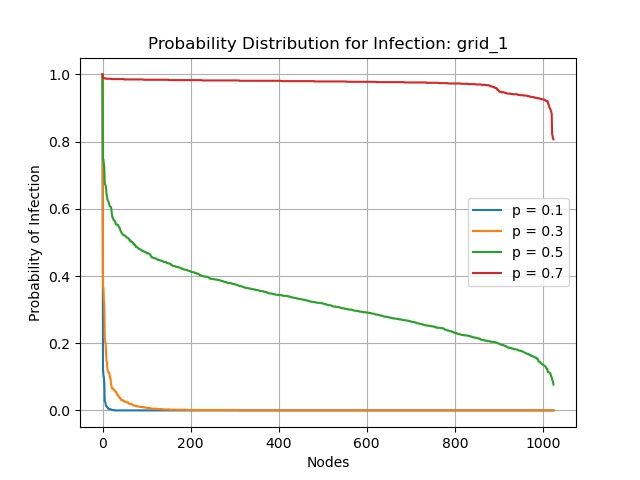
\includegraphics[width=0.33\textwidth]{pdist_grid_1.jpg}
        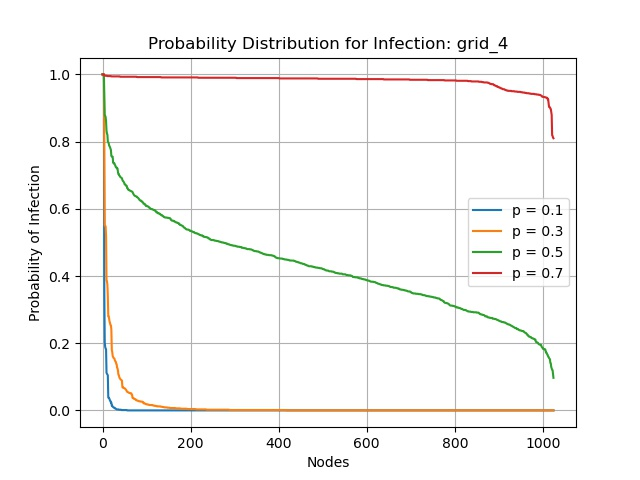
\includegraphics[width=0.33\textwidth]{pdist_grid_4.jpg}\hfill
        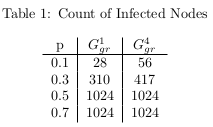
\includegraphics[width=0.3\textwidth]{tab1.png}
    \end{figure} 


    $G^{4}_{gr}$, the grid graph with four infected source nodes, has clearly
    higher infection rates in the 0.1 and 0.3 probability levels. At 0.5 and 
    above, however, both graphs have a significant probability of infection for 
    all 1024 nodes. The following figures show the probability distributions 
    for both graphs.

    %\begin{figure}[htpb]
        %\centering
    %\begin{subfigure}{.5\textwidth}
        %\centering
        %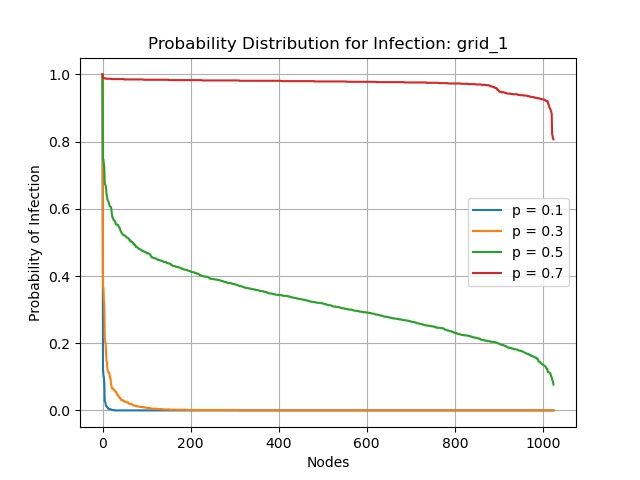
\includegraphics[width=0.6\textwidth]{pdist_grid_1.jpg}
        %% \caption{Probability Distributions $G^{1}_{gr}$}
        %\label{fig:pdist_grid_1-jpg}
    %\end{subfigure}%
    %\begin{subfigure}{.5\textwidth}
        %\centering
        %%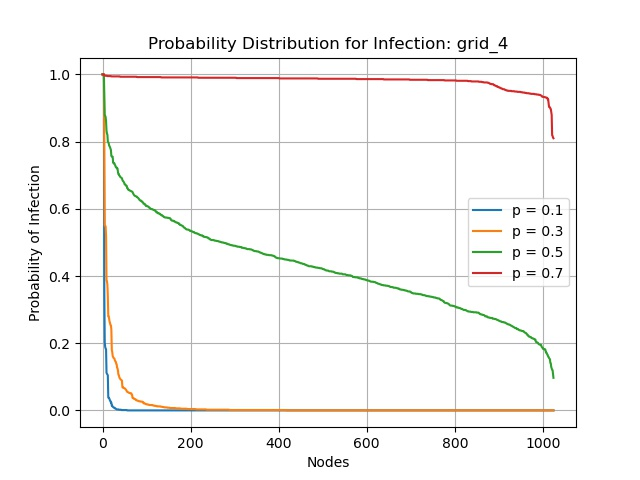
\includegraphics[width=0.6\textwidth]{pdist_grid_4.jpg}
        %% \caption{Probability Distributions $G^{4}_{gr}$}
        %\label{fig:pdist_grid_1-jpg}
    %\end{subfigure}
    %\end{figure}

    The probability distributions for $G^{1}_{gr}$ and $G^{4}_{gr}$ seem to 
    follow the same pattern, but $G^{4}_{gr}$ has a slightly higher absolute
    probability of infection for the same number of nodes. This makes sense as
    the graphs are of the same general structure, so they scale similarly.

    \item \textbf{$G^{1}_{gr}$ and $G^{4}_{gr}$ Days to Infection Distribution}

    %\begin{table}[htpb]
        %\centering
        %\caption{Average Days to Infection}
        %\label{tab:infected_nodes}
        %\begin{tabular}{c | c | c}
        %p & $G^{1}_{gr}$ & $G^{4}_{gr}$ \\ 
        %\hline
        %0.1 & 3.43 & 3.62 \\ 
        %0.3 & 10.89 & 11.17 \\ 
        %0.5 & 30.74 & 27.72\\
        %0.7 & 19.19 & 17.70 \\
        %\end{tabular}
    %\end{table}

    The days to infection are provided here for $G^{1}_{gr}$ and $G^{4}_{gr}$ 
    respectively at each probability level. 0.1: 3.43 and 3.62, 0.3: 10.89
    and 11.17, 0.5: 30.74 and 27.72, 0.7: 19.19 and 17.70.

    The average infection time is pretty close between $G^{1}_{gr}$ and $G^{4}_{gr}$ 
    until we reach the p levels of 0.5 and 0.7. These are also the cases where
    the graph gets more saturated as seen in the previous section. The 
    histograms below show the distribution for each p level.

    \begin{figure}[htpb]
        \centering
        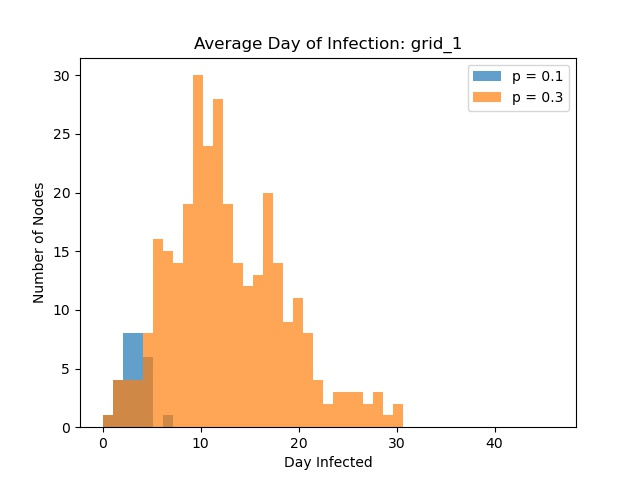
\includegraphics[width=0.3\textwidth]{histogram_grid_1_0_3.jpg}
        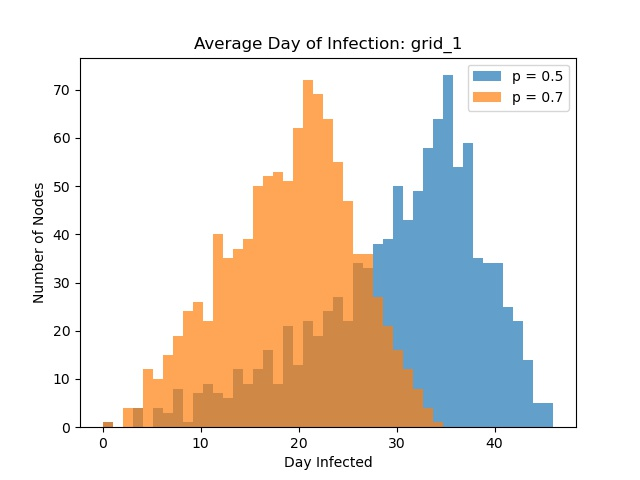
\includegraphics[width=0.3\textwidth]{histogram_grid_1_0_7.jpg}
    \end{figure} 

    \begin{figure}[htpb]
        \centering
        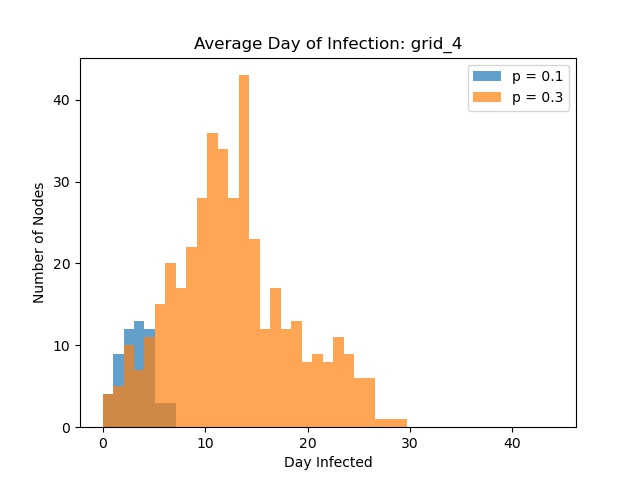
\includegraphics[width=0.3\textwidth]{histogram_grid_4_0_3.jpg}
        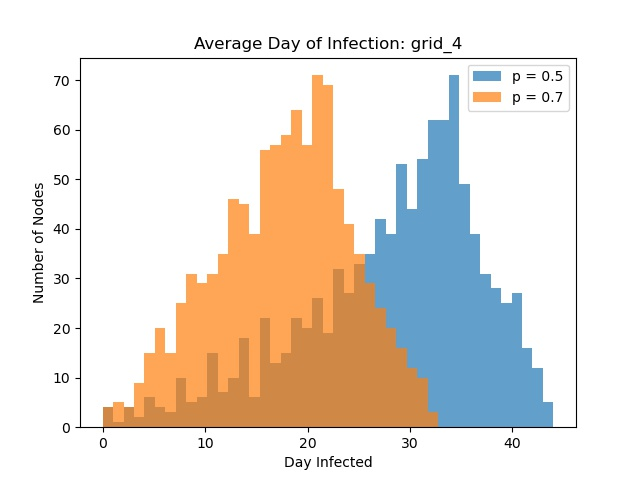
\includegraphics[width=0.3\textwidth]{histogram_grid_4_0_7.jpg}
    \end{figure} 

    The most interesting
    change is from 0.5 to 0.7 where in both graphs the time drops significantly. 
    This is most likely because the graph gets fully saturated in 0.7. In other 
    probability levels the graph is still spreading until the disease dies out 
    at longer time scales.


    \item \textbf{$G^{1}_{gs}$ and $G^{4}_{gs}$ Infected Nodes and Probability Distribution}

    \begin{figure}[htpb]
        \centering
        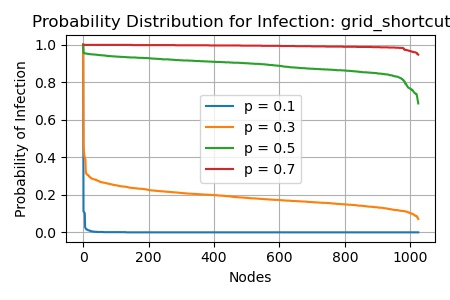
\includegraphics[width=0.33\textwidth]{pdist_grid_shortcut_1.jpg}
        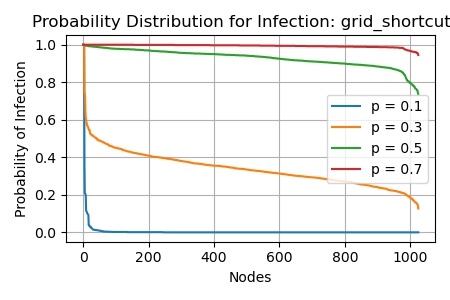
\includegraphics[width=0.33\textwidth]{pdist_grid_shortcut_4.jpg}\hfill
        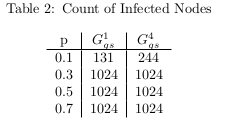
\includegraphics[width=0.3\textwidth]{tab2.png}
    \end{figure} 

    The outcome for $G_{gs}$ is similar to that of $G_{gr}$. The curves on the 
    graph with 4 sources has the curve moved up slightly in the distribution 
    plot. I think the same pattern is followed as both graphs are the same the 
    extra sources just allow for more nodes to be effected at a similar time.

    \item \textbf{$G^{1}_{gs}$ and $G^{4}_{gs}$ Days to Infection Distribution}



    \begin{figure}[htp]
        \centering
        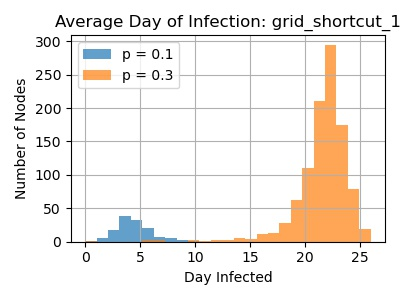
\includegraphics[width=0.3\textwidth]{histogram_grid_shortcut_1_0_3.jpg}
        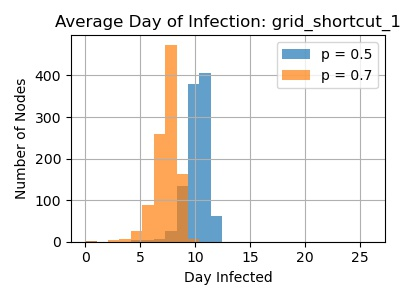
\includegraphics[width=0.3\textwidth]{histogram_grid_shortcut_1_0_7.jpg}
    \end{figure} 

    \begin{figure}[htp]
        \centering
        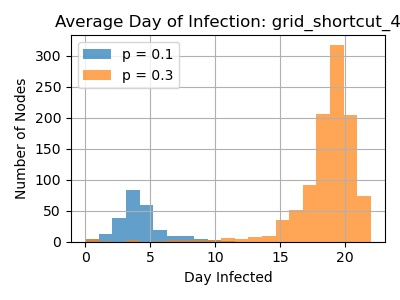
\includegraphics[width=0.3\textwidth]{histogram_grid_shortcut_4_0_3.jpg}
        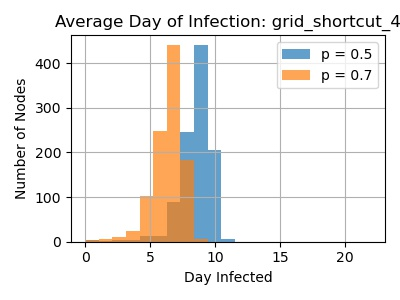
\includegraphics[width=0.3\textwidth]{histogram_grid_shortcut_4_0_7.jpg}
    \end{figure} 

    The days to infection are provided here for $G^{1}_{gs}$ and $G^{4}_{gs}$ 
    respectively at each probability level. 0.1: 4.81 and 4.55, 0.3: 21.29 and
    18.29, 0.5: 10.26 and 8.65, 0.7: 7.63 and 6.61. The pattern here is similar
    to $G_{gr}$ in that higher probabilities see a drop in average time. This is
    because the entire graph is saturated quickly. The spread is accelerated 
    with more sources and more shortcuts.

\item \textbf{$G_{gr}$ and $G_{gs}$ Comparison}

    For the $G^{4}$ graphs, the shortcut graph clearly has more infected nodes
    and higher curves for the probability density functions seen in prior tables
    and figures. The same trend is seen in the $G^{1}$ graphs just with slightly
    lower number of nodes infected and probability curves. This shows that the 
    same structure graph gives the same spreading characteristic, more sources
    give a higher probability of infection with the same shape and shortcuts
    greatly accelerate spread. 

    The same pattern is also seen in time to infection. The saturation point 
    seems to be reached faster as expected in the shortcut graphs and the time 
    to infect is higher before that because the more connected graph makes the 
    spread harder to die and once saturated the times drop much faster.

\item \textbf{Influence of extra shortcut edges}

    The extra shortcut edges both accelerate the spread and make it tougher for
    the spread to die out once it starts. This is evidenced by the upward movement
    in probability distributions in both $G^{1}$ and $G^{4}$ graphs as well as 
    higher spread times before saturation and lower spread times after saturation.

\item \textbf{P=0.5 Impact}
    The difference in infected population when under vs over probability of 0.5 
    makes sense because when over 0.5 a node is now more likely than not to be
    infected. Since these graphs are in a grid shape, most of the near-by nodes
    are also near by to each-others neighbors. If it is more than likely a node 
    will be infected and there are many chances for infection spread becomes 
    almost certain. The spread is exacerbated when shortcuts are added because
    new clusters of infections can start at a distance.
\end{enumerate}

\section{Scale Free Graphs}
\begin{enumerate}
    \item \textbf{Scale Free Networks Comparison}

        For each probability level, both $G^{l}_{sf}$ and $G^{h}_{sf}$ have 
        1000 nodes with a significant chance of being infected - this is all of 
        the nodes in the graph. However, from the probability distributions 
        we can see that there is a significantly higher probability of a number
        of nodes being infected as we go up in propagation probability. The low
        and high degree source graphs show similar shape with the high degree
        having its probability curves shifted up slightly. 

    \begin{figure}[htpb]
        \centering
        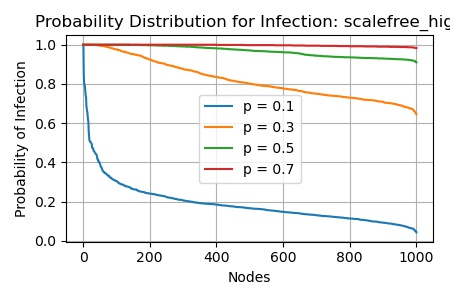
\includegraphics[width=0.33\textwidth]{pdist_scalefree_high.jpg}
        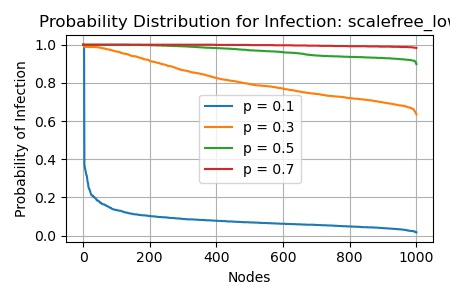
\includegraphics[width=0.33\textwidth]{pdist_scalefree_low.jpg}\hfill
        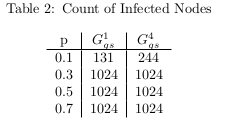
\includegraphics[width=0.3\textwidth]{tab2.png}
    \end{figure} 


\end{enumerate}


%\item \textbf{Most Likely to be Infected}

    %The nodes most likely to be infected are the nodes closest to the source
    %nodes. This makes sense as nodes further away from the sources must have 
    %many nodes between them be infected by chance. Closer nodes are not only 
    %closer directly to the sources but are also closer to other nodes that 
    %are also close to the sources. This raises their probability of infection 
    %greatly in comparison to a node further away.



\end{document}

